\documentclass[11pt, letterpaper]{report}
\input{../../../../report.tex}
\title{General Physics 2: Lab 4 Report}
\date{11/16/24}
\renewcommand{\thesection}{\arabic{section}}
\renewcommand{\headrulewidth}{0pt}
\graphicspath{{../figures}}
\begin{document}
\maketitle
\begin{abstract}
	We investigate Faraday's Law by dropping a bar magnet through a coil of wire. We varied the initial height, the orientation of the poles, and the number of loops of wire. Our resuts generally corroborated those of Faraday's Law.
\end{abstract}
\section{Introduction}
Magnetic flux $\Phi $ can be thought of as the amount of magnetic field $\mathbf{B}$ passing through a given area $A$. Flux can then be calculated using the relationship
\begin{equation}\label{eq:1}
	\Phi =\int_{A}\mathbf{B}\cdot  \mathrm{d} \mathbf{A}
.\end{equation}
Faraday's law states that a change in flux induces a change in electric potential over a coil of wire with $N$ turns, specifically
\begin{equation}\label{eq:2}
	V=-N \frac{\mathrm{d}\Phi }{\mathrm{d}t} 
.\end{equation}
Suppose we drop a bar magnet through a coil of wire. Since the surface $A$ would be horizontal, we only need to account for the vertical component of the magnetic field, since the other components are perpendicular to the normal vectors. Faraday's law in this case yields the relation
\[
	V=-N\frac{\mathrm{d}\Phi }{\mathrm{d}t} =-N\frac{\mathrm{d}}{\mathrm{d}t} \int_{A} \mathbf{B}\cdot \mathrm{d} \mathbf{A}=-N\frac{\mathrm{d}}{\mathrm{d}t} \int_{A} B_z\,\mathrm{d} A=-N\frac{d}{dt}B_zA=-NA \frac{\mathrm{d}B_t}{\mathrm{d}t} 
.\]
It follows that
\[
	\frac{\mathrm{d}B_z}{\mathrm{d}t} =\frac{\mathrm{d}B_z}{\mathrm{d}z} \frac{\mathrm{d}z}{\mathrm{d}t} =\frac{\mathrm{d}B_z}{\mathrm{d}z} v_z(t)
,\]
where $v_z(t)$ is the vertical velocity of the bar magnet. Using this fact, we have
\begin{equation}\label{eq:3}
	V=-N \frac{\mathrm{d}B_z}{\mathrm{d}z} v_z(t)
.\end{equation}
Since $\Phi \propto B_z$ and $A$ is fixed, we know the flux will be at a maximum when $B_z$ is at a maximum. Since the strength of the magnetic field decreases with distance, this maximum happens when the distance is at its minimum. This means we should observe a maximum right before the magnet enters the coil. The magnet then reaches another peak right as the other end of the magnet exits. However, note that the flux is now decreasing, so the induced potential will be the opposite sign for the second peak. Therefore, we can split the $Vt$-graph into two peaks. Furthermore, note that
\begin{equation}\label{eq:4}
	\int_{t_0}^{t_1} V \,\mathrm{d} t=\int_{\Phi(t_0)}^{\Phi(t_1)} -N \,\mathrm{d} \Phi =-N\left( \Phi_1-\Phi_0 \right) 
.\end{equation}
If we consider this to be the first peak, then we are considering $\Phi_0=0$, and $\Phi_1$ to be the maximum of $\Phi $. Similarly, if this is the second peak, then $\Phi_0$ will be the maximum, and $\Phi _1=0$. Using this fact, the integral over the first curve should equal $-N\Phi_{\max }$, and the integral over the second curve equals $N\Phi_{\max }$. This paper uses this relationship to verify Faraday's law, as well as the dependence of equation \ref{eq:3} on both $N$ and $v_z(t)$.
\section{Methodology}
The questions asked by the report necessitate four separate analyses: a control with standardized conditions, an experiment with varying magnet orientations, an experiment with varying numbers of turns, and an experiment with varying $v_z(t)$ values.
\begin{figure}[ht]
	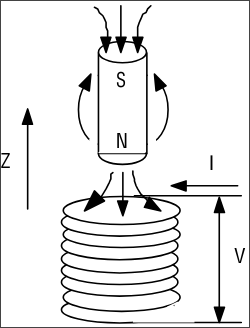
\includegraphics[scale=0.6]{apparatus.png}
	\centering
	\caption{Diagram of Experimental Apparatus}
	\centering
\end{figure}

We will drop a strong bar magnet through a coil of wire, and use technology to measure the induced emf and the value of $N\Phi $ as a function of time, and the maxima and minima of the graphs these values form, and the relevant integrals over the $Vt$-graph. We will then be able to vary the speed by dropping the magnet from different heights, we can vary the number of turns by changing the coil we use, and we can change the magnet orientation by flipping its direction.

In order to miminize error, we dropped the magnet through a plastic tube with a fixed position and orientation. This allowed us to keep the drop coordinates the same by simply dropping it into the top of the tube, as well as preventing the magnet from rotating or moving horizontally as it fell. However, there was tape on the magnet for some reason that caused appreciable friction when dropped with its north end facing updards. To account for this error, we dropped it with the north end facing downwards whenever possible, and ran 3 trials for each data set so we could consider only the average of the data points. We can then give the following list of procedures:
\begin{enumerate}
	\item Set up the experiment with a 1600 turn coil, and drop the magnet with its north end facing downards through it three times. Record the peak value of $N\Phi $, and the integrals over the two peaks of $V$.
	\item Repeat step 1, but with the north end of the magnet facing upwards.
	\item Repeat step 1, but with different coils with different numbers of turns.
	\item Repeat step 1, but with different initial heights of the magnet.
\end{enumerate}
\section{Data}
\subsection{Data Record}
Unless otherwise specified, the initial height is 0.226$m$, the orientation is down, and the number of turns is 1600.
\begin{center}
	Table 1: Control\label{tab:1}\vspace{5pt}\\
	\begin{tabular}{rrr}
	\toprule
	Area 1&Area 2&$N\Phi_{\max }$ (Turns$/m^2$)\\
	\midrule
	0.1316&-0.1339&-0.1332\\
	0.1325&-0.1341&-0.1336\\
	0.1320&-0.1342&-0.1333\\
	\bottomrule
\end{tabular}\vspace{20pt}\\
Table 2: Varying Magnet Orientation\label{tab:2}\vspace{5pt}\\
\begin{tabular}{rrrr}
	\toprule
	Area 1&Area 2&$N\Phi_{\max }$ (Turns$/m^2$)&Up/Down\\
	\midrule
	-0.1301&0.1329&0.1327&Up\\
	-0.1301&0.1342&0.1331&Up\\
	-0.1310&0.1332&0.1332&Up\\
	\bottomrule
\end{tabular}\vspace{20pt}\\
Table 3: Varying Number of Turns\label{tab:3}\vspace{5pt}\\
\begin{tabular}{rrrr}
	\toprule
	Area 1&Area 2&$N\Phi_{\max }$ (Turns$/m^2$)&Turns\\
	\midrule
	0.0320&$-0.0328$&$-0.0321$&400\\
	0.0331&$-0.0328$ &$-0.0322$ &400\\
	0.0312&$-0.0322$ &$-0.0315$ &400\\
	\bottomrule
\end{tabular}\vspace{20pt}\\
Table 4: Varying Initial Height\label{tab:4}\vspace{5pt}\\
\begin{tabular}{rrrr}
	\toprule
	Area 1&Area 2&$N\Phi_{\max }$ (Turns$/m^2$)&Initial Height (m)\\
	\midrule
	0.1288&$-0.1336$ &$-0.1325$ &0.195\\
	$0.1228$ &$-0.1337$ &$-0.1309$ &0.169\\
	0.1328&$-0.1352$ &$-0.1334$ &0.300\\
	\bottomrule
\end{tabular}
\end{center}
\subsection{Data Analysis}
Our analysis will consist largely of responses to questions asked by the report instructions, and we will indicate what question we are responding to at all appropriate points.

\textbf{Question 1.} Recall Faraday's Law (\ref{eq:2}). Since $V\propto -\frac{\mathrm{d}\Phi }{\mathrm{d}t} $, we know that when $\Phi $ is increasing, $V<0$; when $\Phi $ is decreasing, $V>0$; when $\Phi $ is at a maximum, $V=0$. Since $\Phi $ depends on $B_z$ which depends on distance from the coil, the shape of its graph is similar to a bell curve. This means for the first half, its derivative is positive, so $V$ goes down for a while. Then it comes back up2 and hits $0$ when the magnet is perfectly centered in the coil, since the flux is at a maximum here. The distance then begins to decrease, so $\Phi $ goes down, and $V$ is positive.

\textbf{Question 2.} The magnitudes of the first peaks are always smaller than the magnitudes of the second peaks, with a single exception. This could possibly be due to contributions from the Earth's magnetic field, but since the bar magnet is much stronger than the Earth's field, it's likely this only accounts for a small fraction of the difference. Most of the difference comes from equation \ref{eq:3}, where we noted $V\propto v_z(t)$. Since the magnet accelerates through the coil, it has a higher velocity by the time it reaches its second peak, so $v_z$ will be higher, meaning $V$ is higher for the second peak.

\textbf{Question 3.} Using the previous logic, we expect the second peak to have more area. The magnet is moving faster throughout the second curve, meaning the flux is changing faster, meaning $V$ will have a greater magnitude by equation \ref{eq:2}.

\textbf{Question 4.} The magnetic field goes out from the north pole and goes into the south pole. This means when the north pole is facing down, the magnetic field is moving outwards through the coil and generating a positive flux. However, when the south end faces down, the field is moving towards the magnet, generating a negative flux. Another way to generate this is to shoot the magnet upwards through the coil with the north end facing down, or we can flip the coil upside down and drop the magnet with the north end facing down.

\textbf{Question 5.} First, we will consider the areas under the curve. Note that the averages of areas 1 and 2 in table \hyperref[tab:1]{1}  are 0.1320 and 0.1341, respectively. The same values for table \hyperref[tab:3]{3}  are 0.0321 and 0.0326. Since we went from 1600 turns to 400 turns, by equation \ref{eq:2} we would probably expect these values for table \hyperref[tab:1]{1}  are about $4$ times that of table \ref{tab:3}. We have
\[
	\frac{0.1320}{0.0321}=4.112,\qquad \frac{0.1341}{0.0326}=4.113
.\]
Since the deviations from the expected value are basically the same, and since they are very small, it's likely that the area under the curve is linear in $N$.

Now consider the peaks of $V$.
\begin{center}
	Table 5: Peaks in $V$\label{tab:5}\vspace{5pt}\\
	\begin{tabular}{rrr}
		\toprule
		Peak 1&Peak 2&Turns\\
		\midrule
		5.1810&5.9940&1600\\
		5.7250&6.4510&1600\\
		5.4510&6.3880&1600\\
		1.3580&1.5720&400\\
		1.3100&1.4690&400\\
		1.1240&1.2690&400\\
		\bottomrule
	\end{tabular}
\end{center}
The averages in peak 1 and peak 2 for $1600$ turns are 5.4523 and 6.2790, respectively. The same values for 400 turns are 1.2640 and 1.4367, respectively. We have
\[
	\frac{5.4523}{1.2640}=4.3134,\qquad \frac{6.2790}{1.4367}=4.3696
.\]
Once again, these values are fairly close to the theoretical value of $4$, and the deviation from the theoretical is about the same for both. Therefore, we conclude that the theoretical value likely holds, but we will return to these assumptions in the error analysis section.

\textbf{Question 6.} To answer this question, we will first calculate the speed of the magnet as a function of the distance it has fallen. Recall that gravitational potential energy is  $U=mgh$, and kinetic energy is $\frac{1}{2}mv^2$. We have
\begin{equation}\label{eq:5}
	v=\sqrt{2gh} 
.\end{equation}
Using this relationship, we can plot the peaks and areas as a function of speed.
\begin{figure}[ht]
	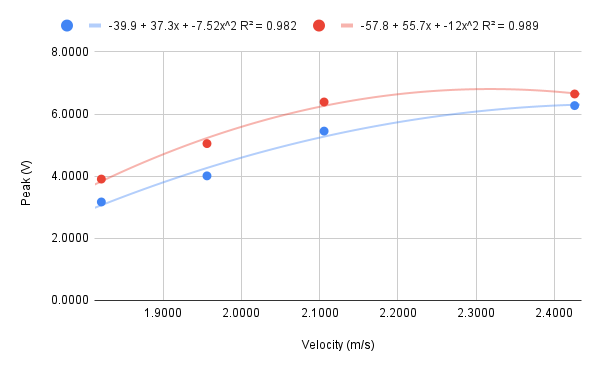
\includegraphics[scale=0.5]{chart3.png}
	\centering
	\caption{$v_z(t)$ vs Peaks 1 and 2}\label{fig:2}
\end{figure}

Using figure \ref{fig:2}, we can see that the relationship between the maxima of $V$ is not linear in $v_z(t)$, and is likely quadratic.

\begin{figure}[ht]
	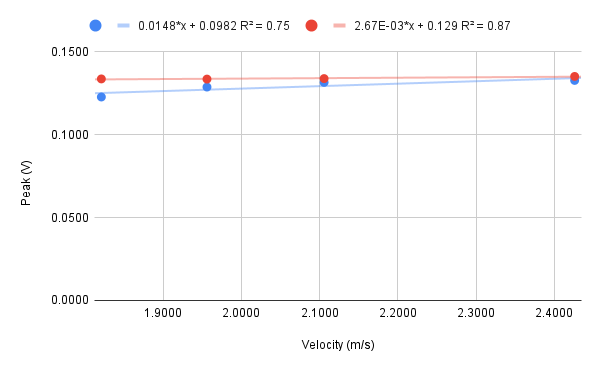
\includegraphics[scale=0.5]{chart2.png}
	\centering
	\caption{$v_z(t)$ vs Areas 1 and 2}\label{fig:3}
\end{figure}

Using figure \ref{fig:3}, we can determine that the relationship between velocity and the areas under $V$ are linear. This lines up with equation \ref{eq:3}, which claims that the integral over $V$ will be proportional to the integral over $v_z(t)$.

We will now identify  the magnitude of $B_z$ for our magnet. The cross-sectional area of the magnet was $\pi \cdot 0.01^2$ meters. The magnetic field in the coil was approximately confined to the magnet, so our area $A$ becomes this area. By equation \ref{eq:4},
\[
	\Phi_{\max }=\int_{A}\mathbf{B}\cdot  \mathrm{d} \mathbf{A}=AB_z=B_z\left( \pi  \cdot 10^{-4} \right) 
.\]
We will use the value of $\Phi _{\max }$ from our first trial, since it went very well. We have
\[
	B_z=\frac{0.1332\left( \frac{1}{1600} \right) }{\pi \cdot 10^{-4}}=0.2650\text{T}
.\]
Therefore, the magnetic field of our magnet was $0.2650$T.

\textbf{Question 7.} Note that $5.5\cdot 10^{-5}\ll2.65\cdot 10^{-1}$. Therefore, the Earth's magnetic field should have no appreciable effect on the results.
\section{Discussion}
It's important to note that our experiment was not without error. When dropping the magnet when oriented upwards, there was extremely appreciable friction between the tape and the tube sidings. Furthermore, we used a very nonexact method of measuring the drop height, and there were some instances where the computer would continue collecting data after the magnet had hit the ground, skewing the second values to be higher than the first. This means our results are likely not correct in general, especially those of figure \ref{fig:2}, which I expected to be linear, and for which I could find no justification for why it appeared nonlinear.
\end{document}
